
\documentclass[letterpaper,twocolumn,10pt]{article}
\usepackage{usenix}
\usepackage{graphicx}
\usepackage{endnotes}
\usepackage{float}      % force fixed figure placement
\usepackage{subfloat}
\usepackage{amsmath}
\usepackage{algorithm}
\usepackage[noend]{algpseudocode}

\graphicspath{ {./} }

\begin{document}

%don't want date printed
\date{}

%make title bold and 14 pt font (Latex default is non-bold, 16 pt)
\title{\Large \bf KM : Effective Data Tracing In Distributed Systems}

%for single author (just remove % characters)
\author{
{\rm First Name}\\
First Institution\\
\and
{\rm Second Name}\\
Second Institution
% copy the following lines to add more authors
% \and
% {\rm Name}\\
%Name Institution
} % end author

\maketitle

% Use the following at camera-ready time to suppress page numbers.
% Comment it out when you first submit the paper for review.
\thispagestyle{empty}


\subsection*{Abstract}
Modern Internet services often involve large and complex distributed systems
with data scattered around. As the number of services grows and data access
scenarios get varied, important data might get leaked or stolen with no
knowledge of the system administrators. In this paper we propose KM, a system
which is used to trace data access and transfer in distributed systems. We
present the model for tracing how data are accessed and transferred, showing
that this model can succinctly capture users behaviors and thus can be used
% TODO replay scenarios ??? wording correct?
to replay scenarios where data are leaked or stolen. We also present a
efficient implementation of KM and show that with proper sampling strategies
our implementation can have negligible impact on existing services. 

\section{Introduction}
Data access control and monitoring in complex distributed systems have been a
% TODO more papers here
real world concern~\cite{cloudComputing:2010} but have not yet gathered enough
attention. Large internet companies which provide heterogeneous services
often have their data stored in different data centers but the technologies
they use to process these data, such as Mapreduce~\cite{MapReduce:2008} and
Spark~\cite{Spark:2015}, are built with no security in mind, making it hard to
precisely grant data access permission to relevant users and, in case of data
being stolen, trace how the data are transferred. In this paper we try to
mitigate this situation by using a model to capture user program behaviors
and design a system called \textit{KM} to efficiently collect information of
interest such that we can trace how a piece of data is accessed and
transferred within or across machines and then probably stolen (i.e., copy
into a USB stick or send to some remote machine). 

The goal of KM is to track data access and transfer. The term \textit{event}
is used to describe any activity related to a piece of data. An
\textit{event} is modeled with a triad \textit{(Subject, Action, Object)}. To
succinctly model program behaviors, \textit{event}s are classified into three
categories: \textit{file event}s, \textit{network event}s and \textit{process
event}s. Examples of \textit{file event}s include opening, reading and
writing files; examples of \textit{network event}s are binding a socket,
connecting to remote machines and accepting incoming connections; examples of
\textit{process event}s are forking subprocesses and executing executables
via the \textit{execve()} system call. As will be shown below, these three
classes of events are sufficient to model program behaviors. 

The whole system is designed to be configurable. Strategies can be add or
delete at anytime using a \textit{KMctl} program or with the corresponding
API. Therefore one can set up a central configuration service to manipulate
% TODO maybe it is not that accurate to call that 'configuration' strategy
% TODO and the word `strategy' needs to be considered more
strategies used by every single machine. These strategies include turning the
tracing system on and off, controlling sampling rate and adding a file to be
tracked. Note that our system is \textit{data-oriented}, which mean that
instead of collecting all events information, it will only collect
information related to the data of interest. If during file transfer some
intermediate files are not in our list (\textit{e.g.}, process A read file
\textit{a} and write to file \textit{b}. Process B read from file \textit{b}.
We have file \textit{a} in our list, but the intermediate file \textit{b} is
not in our list), we will add the intermediate files to the global
configuration at runtime, which can then be seen by the whole system. 

Besides, we have implement a utility called \textit{hotpatcher} which can be
used to insert a dynamic shared object (DSO) into a user program, so that one
can deploy this tracing system without having to reboot machines and
affecting existing services. This utility can also be used to
\textit{partially} deploy the tracing system, which is very helpful at the
time of testing.\\

Under the hood we have interposition in libc, using the LD\_PRELOAD
technique~\cite{LDPRELOADKrentel:2013, LDPRELOADLee:2011, LDPRELOADSaito:2005}
or using the \textit{hotpatcher} utility program
described above. Whenever a program try to operate on the data of interest
(e.g, reading or writing), a piece of information, which is necessary for
data tracing afterward, will be collected by our interposition code and then
sent to a message queue in a piece of shared memory. The shared memory is set
up by a daemon called \textit{KMagent} when it is started (usually at boot
time) and is shared among all processes at that single machine.
\textit{KMagent} is the consumer here, continuously polling the shared
message queues and collecting data, whereas all the other processes are
producers. The message queue in shared memory is wait-free and operations on
it are guided by a protocol to make them efficient and safe, affecting no
existing services. As will be demonstrated below, with the current
implementation, the overhead within a single event is about 1\textit{us} on 
% TODO machine specification
our[-- TODO machine specification --]. With proper sampling strategies, we
show that our implementation have only negligible impact on file events, 10\%
overhead on process event and 10\% overhead on network event. 

Periodically a central service try to pull from all machines to collect newly
% TODO and then analyse those data offline or use streaming stategy
generated data. We use a \textit{bulk mode}~\cite{CACMDean:2013} to make this
operation cheap. Besides, our system is \textit{data-oriented}, which makes
% TODO explain this "data-oriented", because mostly people will forget our
% focuse on "data-oriented" (including me)
the volume of collected data small, thus placing only low burden on the
system.\\

There has already been lots of works in using tracing techniques to gather
information about distributed system behaviors~\cite{magpie:2004, magpie:2003,
pinpoint:2002, xtrace:2007, dapper:2010}.  However, those works almost all
focus on performance analysis and trouble-shooting. Most of them are targeted
to some specified program (\textit{e.g.}, web server)~\cite{magpie:2004,
magpie:2003} and require help from the operation system kernel. Compared to
them, our attention is on tracking how data is accessed and transferred, and
then determine whether those operations are legitimate. Our system can affect
\textit{every} process on a machine with sufficiently low overhead. With the
implementation in userspace, the whole system is also easy to test and
customize. We draw some ideas from~\cite{BackTraceKing:2003,
BackTraceKing:2005}. Our model can capture user behaviors precisely. Along the
way, we design an simple but efficient system which imposes negligible impact
on existing services.\\

To summarize, our contributions are:
\begin{enumerate}
    \item a model that can precisely capture program behaviors and track how
        a piece of data are accessed and transferred.
    \item a system with efficient implementation which impose negligible
        impact on existing services.
    \item the ability to query and control strategies used in the system and
        the ability to deploy the whole system while requiring no reboot.
\end{enumerate}

The structure of this paper is as follows: in section 2 we present the model
we use to capture user behaviors and tracing data transfer. We then show
details of our implementation in section 3, along with its strategies. In
section 4, we present some experiments carried out on a small cluster and
show that it has negligible impact on existing services. We discuss related
work and future work in section 5 and section 6 respectively and then
conclude in section 7.

\section{Model} \label{sec:themodel}

% note: you can also use the wonderful epsfig package...
\begin{figure}[t]
    \centering
    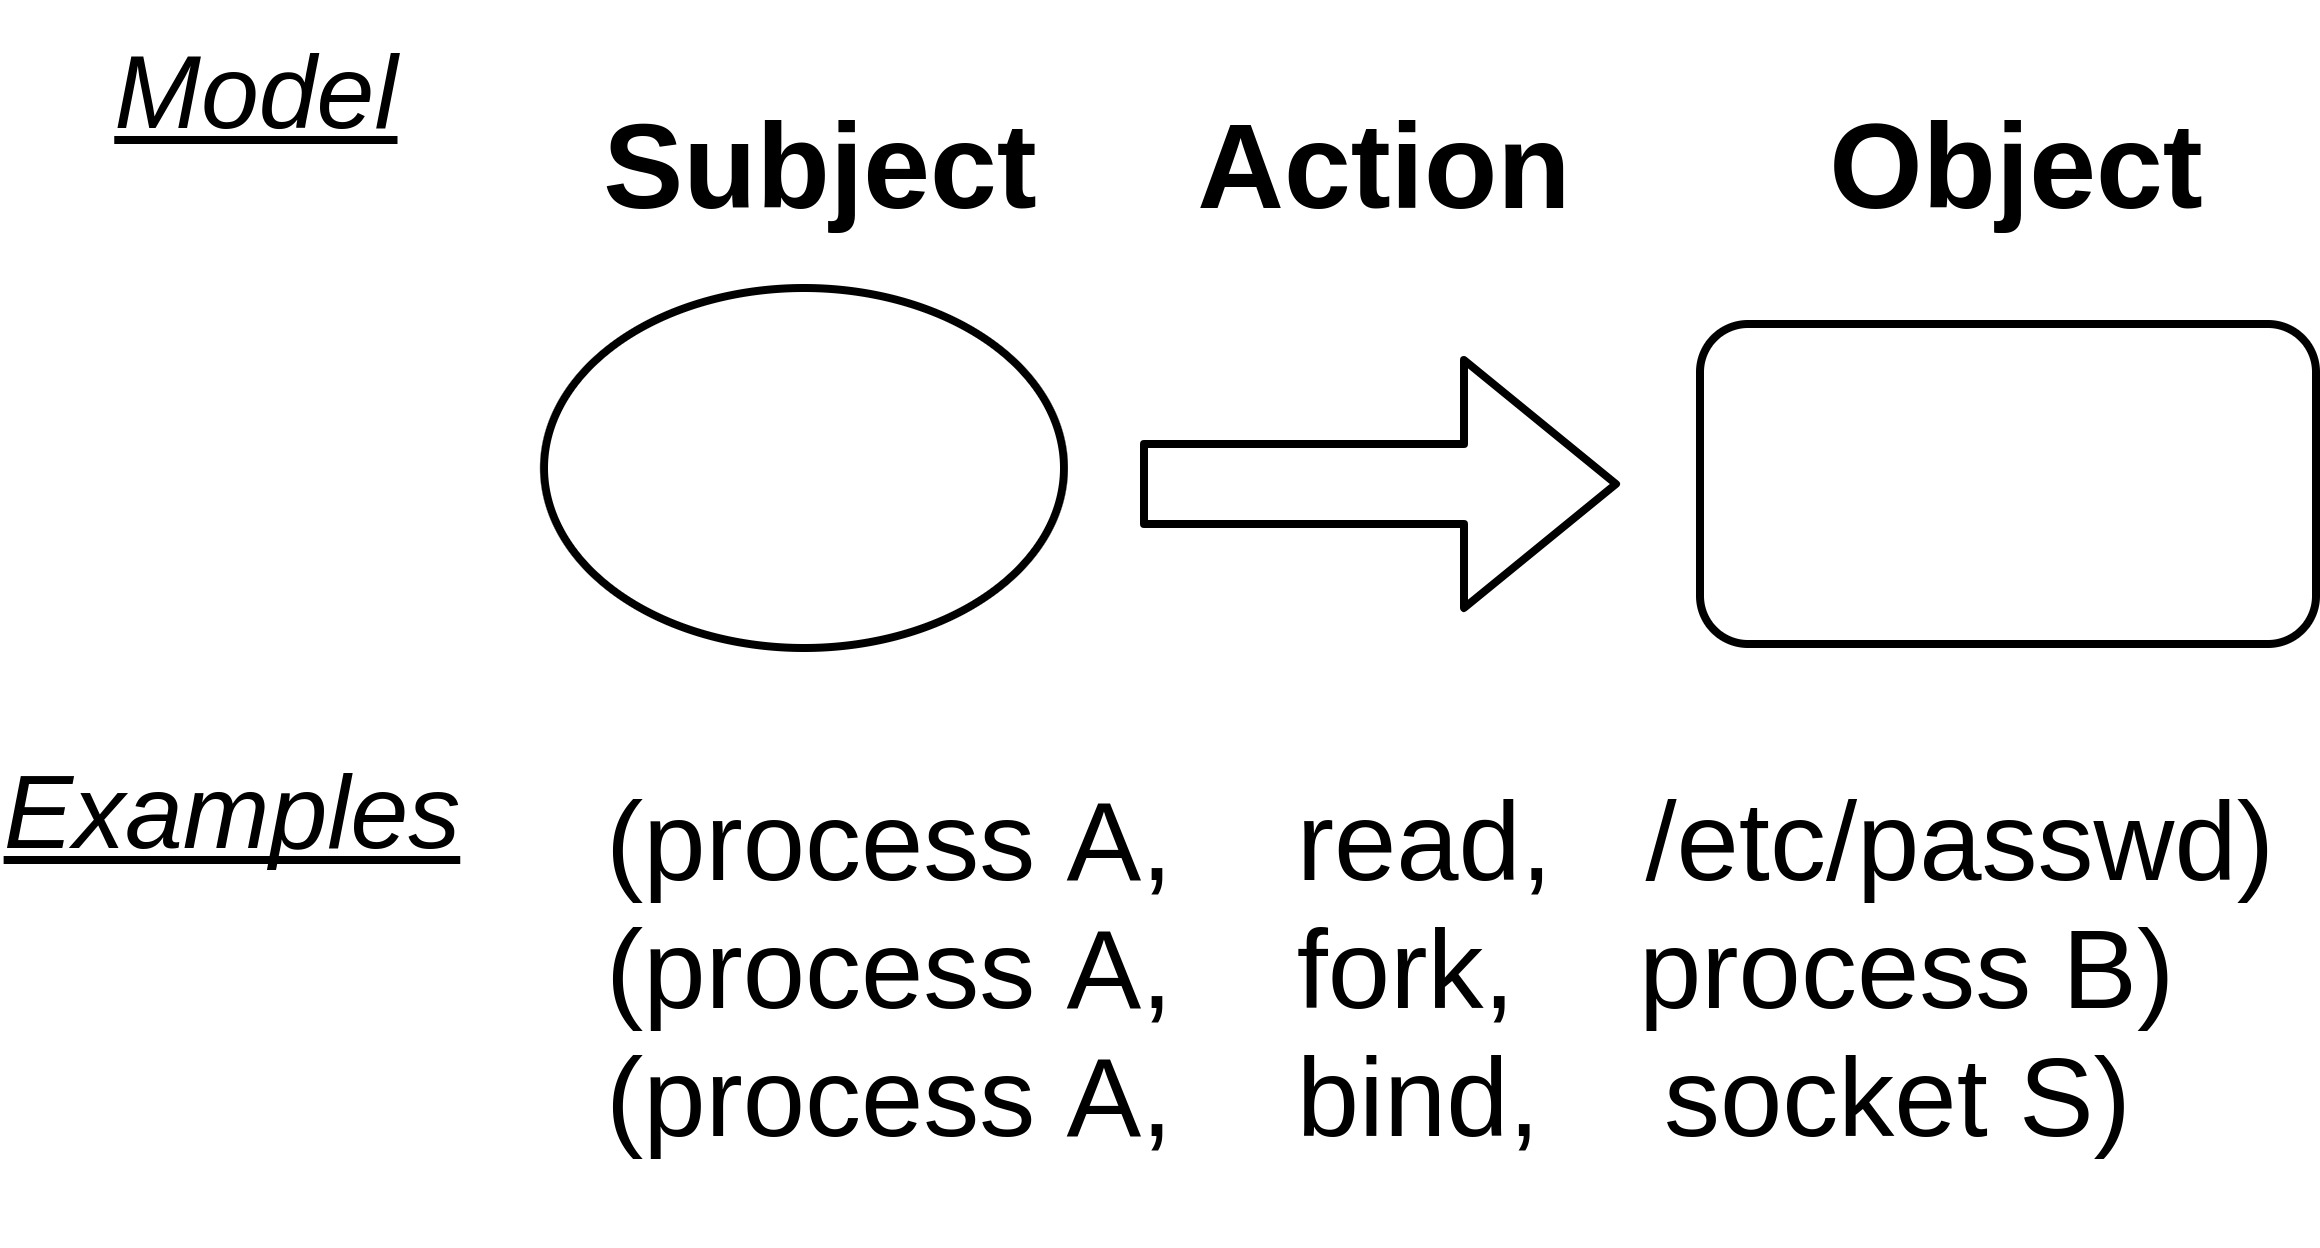
\includegraphics[scale=0.08]{saomodel.eps}
    \caption{The Subject-Action-Object Model}
    \label{fig:saomodel}
\end{figure}

In this section we present the model used by KM. In KM, any activity related
to a piece of data is called an \textit{event}, which is modeled with a triad
\textit{(Subject, Action, Object)}, as shown in Figure~\ref{fig:saomodel},
with examples. All events are classified into three categories: \textit{file
event}s, \textit{network event}s and \textit{process event}s. If process A
read a file \textit{/etc/passwd}, this ``read" operation will be recorded by
our system which then emits a triad \textit{(process A, read, /etc/passwd)}.
Similarly, if process A calls \textit{fork(2)} (and probably communicate with
its child process afterward), this ``fork" operation will also be recorded
and finally a triad \textit{(process A, fork, process B)} will be emitted by
the system. Same for the network event when a process A bind to a socket S. 

Since most Unix-like systems (\textit{e.g.}, Linux) treat most things as
files, if we can record all the relevant file events, we can then capture
most of the key operations related to some particular piece of data, such as
reading a file and sending it over a socket, thus being confident in knowing
how a file is accessed and transferred. If we also have 
% TODO Is "at hand" a good phrase? is
processes events at hand, we can know how processes interact with each other
and build more confidence in file transfer within a single machine. Moreover,
with network events, we can know how a file is transferred across machines.
Therefore, with information of these three types of events, we can capture
user behaviors on some piece of protected data and trace its transfer route
in a distributed system.\\

% add a * to make this figure span across two columns.
\begin{figure*}
    \centering
    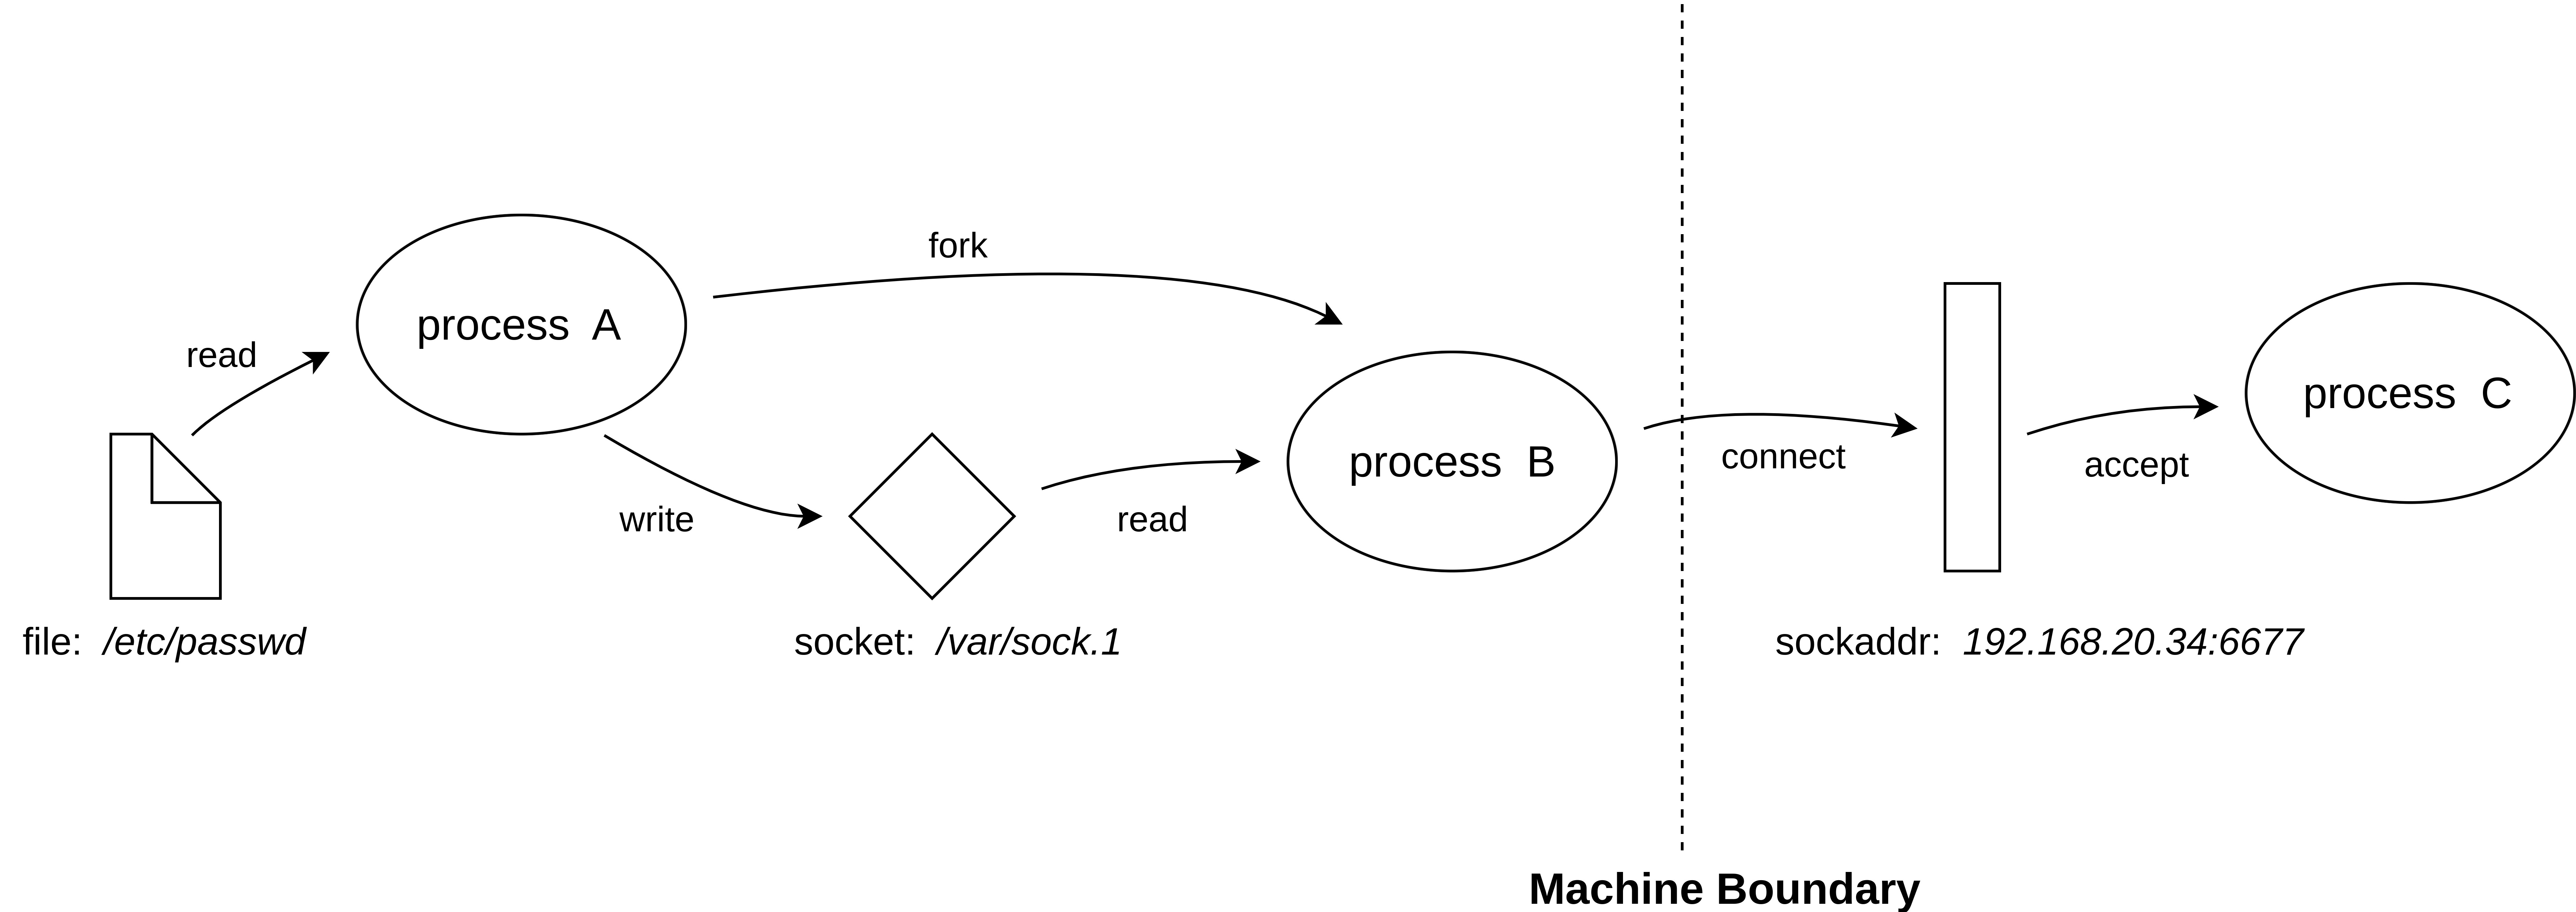
\includegraphics[scale=0.06]{filetransfermodel.eps}
    \caption{left: file access and transfer in a single machine. right: distributed system }
    \label{fig:filetransfermodel}
\end{figure*}

% model on a single machine
\noindent
\textbf{Trace on The Same Host} On a single machine, if a file is under
monitor, then any access of it by any process will be recorded by our
system. Subsequent file operations by that particular process (\textit{e.g.},
writing to a file in \textit{/tmp} or send it over a socket) will also be
recorded. These records are all emitted as file events. Because processes
mostly interact with their child processes or parent processes, we also
record function calls such as \textit{fork(2)}, \textit{clone(2)} and
\textit{execve(2)} and emit those records as process events. Combining file
events and process events, we can build a clear picture of how a protected
file are accessed and transferred on a single machine, as shown at the left
of Figure~\ref{fig:filetransfermodel}.\\ 

% model across machines
\noindent
\textbf{Trace Across Hosts} In a distributed system, processes in different
machines usually communicate with each other through network operation such
as \textit{connect(2)} and \textit{accept(2)}. These operations are all
recorded by KM which then emits them in the form of network events. These
network events bridge the gap of file transfer between different machines, as
shown at the right of Figure~\ref{fig:filetransfermodel}.\\

Note, however, that while we use only a triad \textit{(Subject, Action,
Object)} to model events, the data collected for each event contain sufficient
information, such as execution time and process name, to chain up together all
relevant events within a host and across hosts. A detail description of this
process will be given in section \ref{sec:fwtracing}.

% Now we are going to add in the probability model (note the "build more
% confidence words above")
TODO probability model

\section{Implementation}

\subsection{System Overview} KM is implemented in userspace and relies on the
LD\_PRELOAD mechanism of the dynamic linker. In short, whenever a program
starts, the dynamic linker will load the shared libraries listed in the
LD\_PRELOAD environment variable before any other libraries that the program
depends on, including libc.so. After the dynamic linker is done with symbols
relocation, symbols exported by shared libraries in LD\_PRELOAD will ``shadow"
those with the same names in libc.so. Because libc is the common runtime which
provides system call wrappers and common routines for application to interact
with the operating system and most programs depends on libc.so, we can use
this feature to add wrappers around libc's and insert some interposition code
between user program code and libc. This is illustrated in
Figure~\ref{fig:ldpreload}.

% use `H' to fix figure placement, with help from the `float' package
\begin{figure}[H]
    \centering
    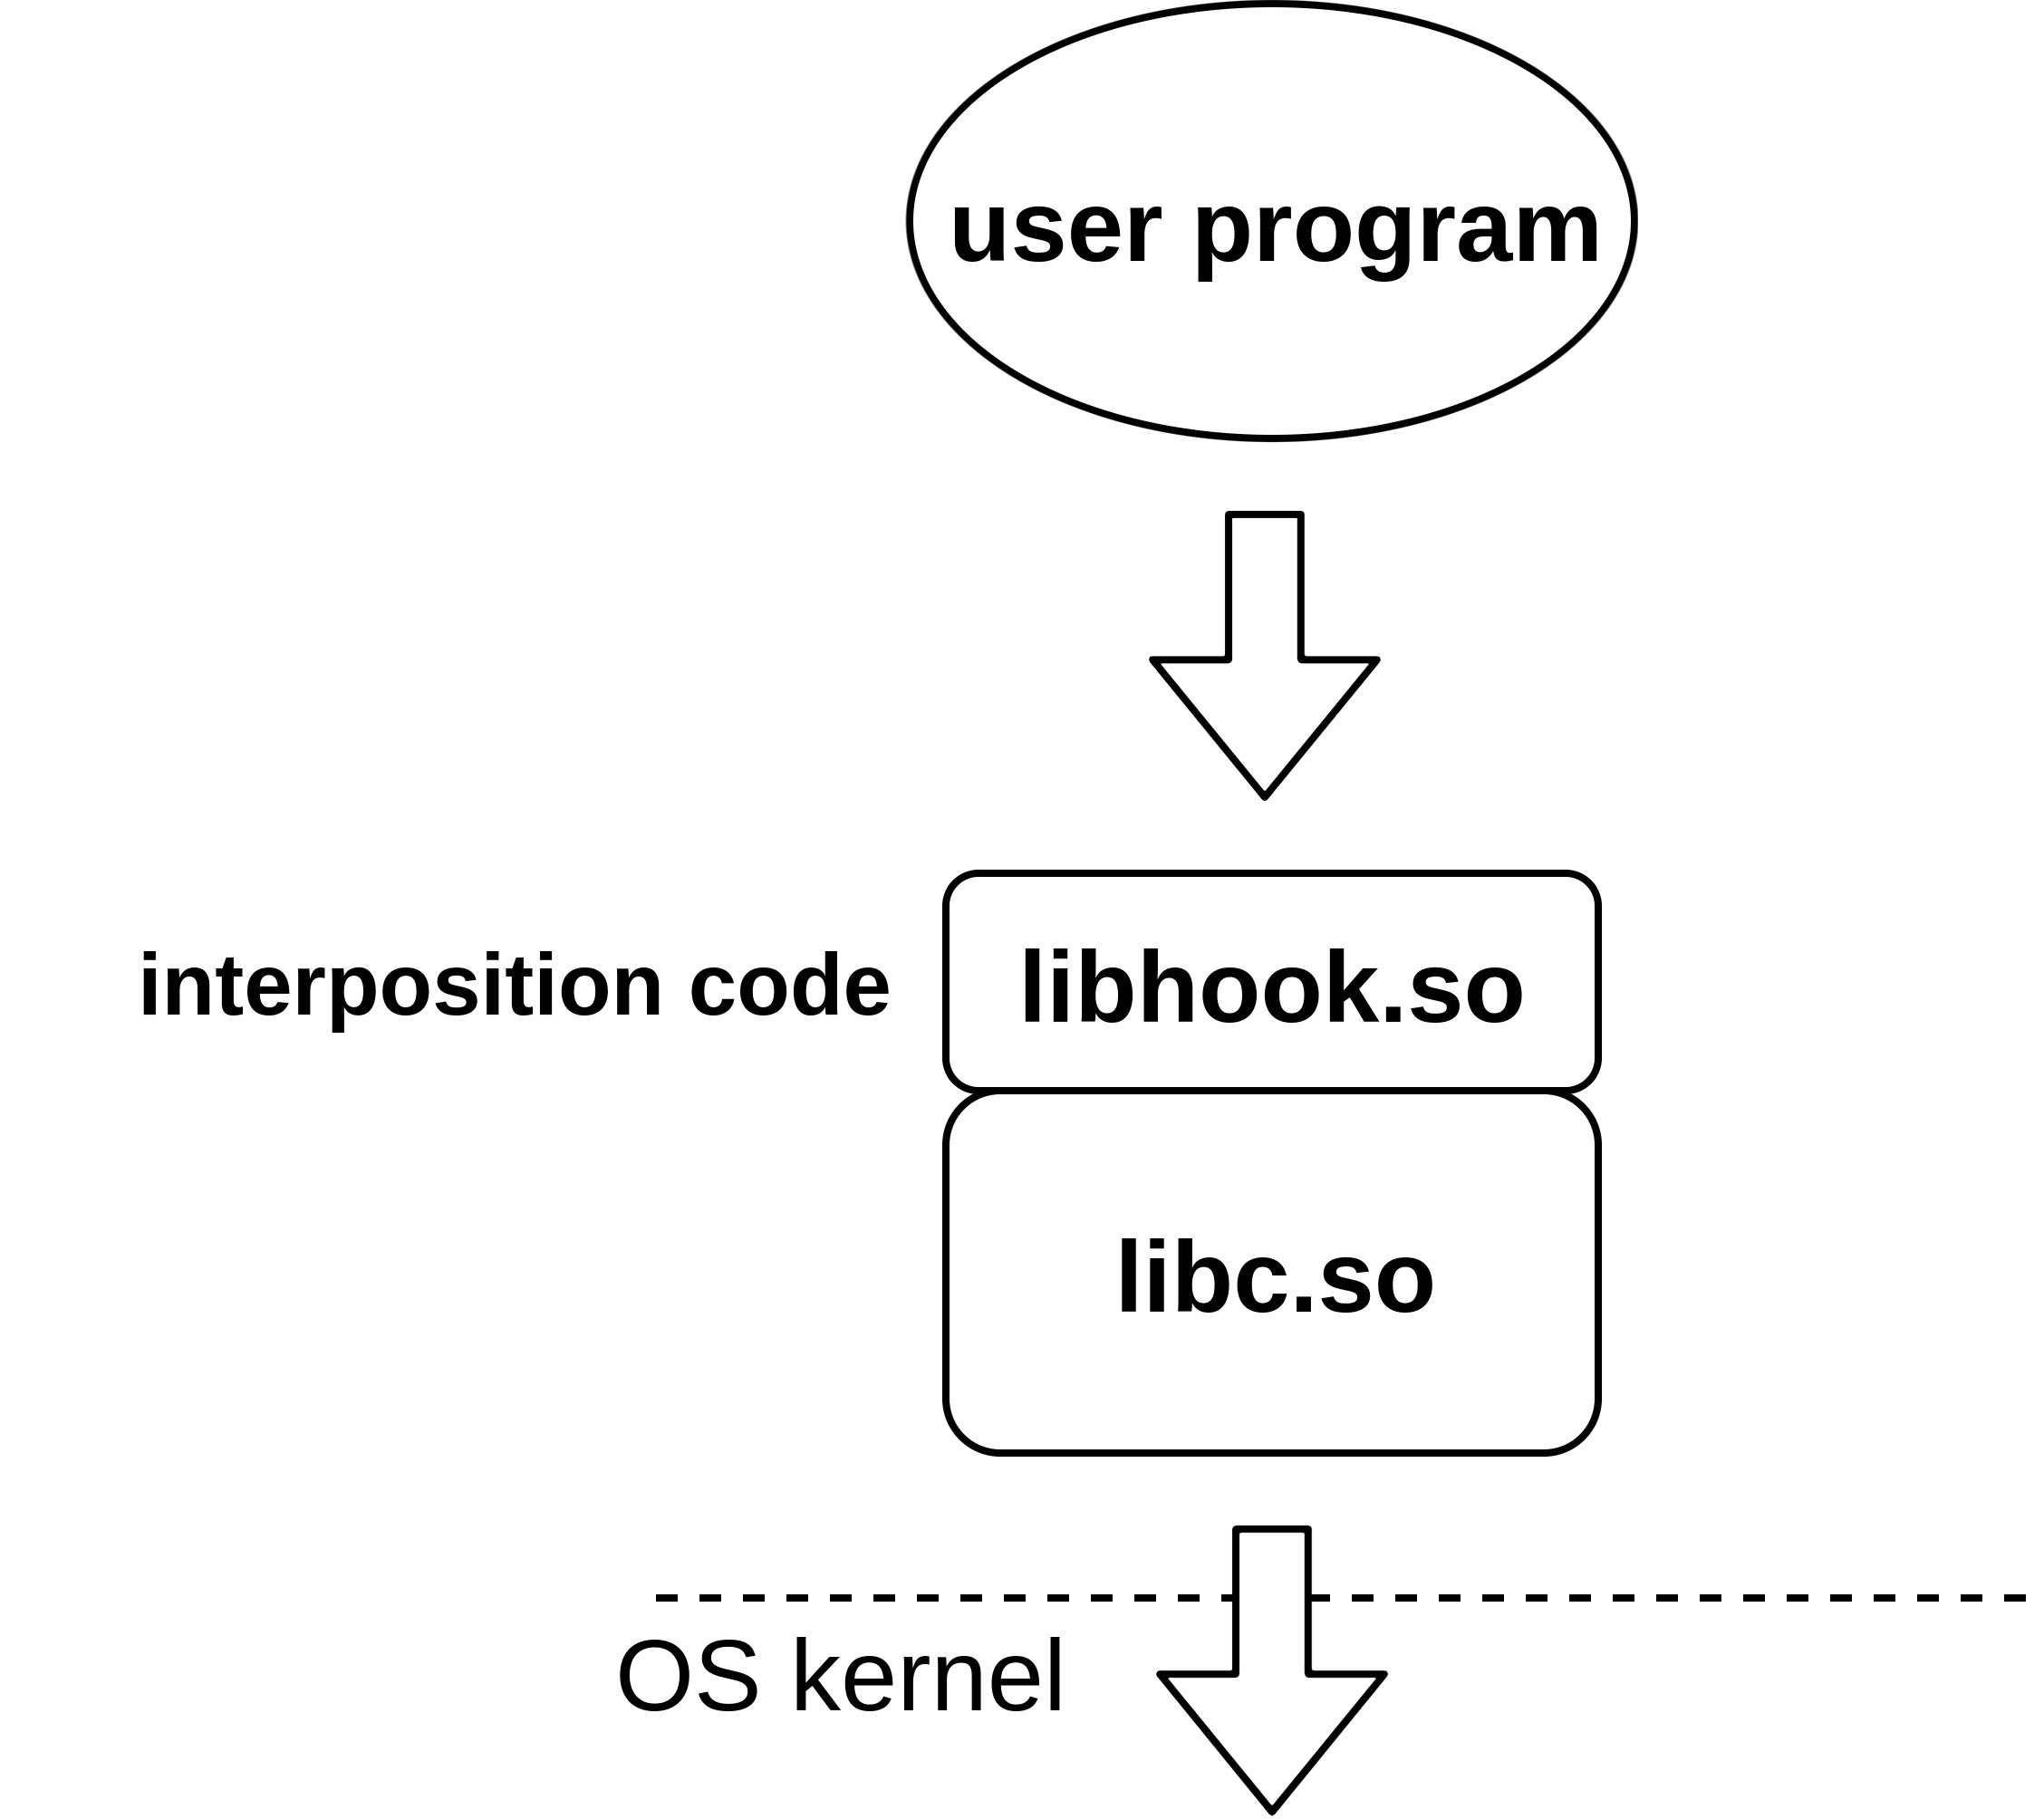
\includegraphics[scale=0.07]{singlemachine.eps}
    \caption{The LD\_PRELOAD Mechanism}
    \label{fig:ldpreload}
\end{figure}

This schema is common for libc interposition~\cite{LDPRELOADLee:2011}. However, to
make the implementation safe and efficient is not easy. To make it safe, one
have to adhere strictly to the semantic of every API and every piece of code
should be multithread-safe and async-signal-safe. To make it efficient, only
a small piece of code should be added, because many system calls
(\textit{e.g.}, \textit{accept(2)}) will be invoked very frequently. In order
to achieve these, our interposition code in every function wrappers contain
only a few memory operations. This requires transforming most operations to
memory operations. Therefore, a piece of shared memory is set up by the
\textit{KM agent} at the very beginning and attached by every hooked user
program at program startup. After that, all operations, such as sending
function invocation record, can be done through this shared memory. Also,
there are configuration rules in the shared memory, which can be referenced
by interposition code in every user program.\\ 

At program startup, the constructor of \texttt{libhook.so} will be invoked,
which then allocates a piece of memory in the process space of the current
process. This piece of memory is used to hold relevant information of the
current process that may be needed afterward. The relevant information will
be gathered by reading the \texttt{/proc} filesystem (\textit{e.g.}, to get
process starttime) or invoking proper system calls (\textit{e.g.}, getpid()). 

In the interposition code, all our wrappers will perform configuration
checking, gather information about this particular function invocation and
then send those information to the in-shared-memory message queues, which
will be described in section \ref{sec:effimq}. All these operations involve
only some memory operations. Below is a simplified wrapper for
\textit{read(2)}: 

{\tt \small
\begin{verbatim}
int read_wrapper(int fd, void *buf,
                 size_t count) {

    int fd = read_original(fd, buf, count);
    if(fd < 0)
        return fd;
    if(!read_specified())
        return fd;
    if(!check_conf())
        return fd;
    send_read_info();
    return fd;
}
\end{verbatim}
}

% make it clear that it's a continuation of the preceding text.
\noindent
Basically it invokes the original \textit{read(2)} in libc first, and then
check configurations in shared memory to see whether or not this file is
under monitor and thus operations upon it should be recorded. Because the
configuration checking is done through the shared memory, which is attached
at program startup, and we employ some hashing techniques (described in
section \ref{sec:optm}) for fast searching, it should be fast and safe. After
that a traid of file event, as described above in section \ref{sec:themodel},
will be send to message queues in shared memory. Note that we do not have to
make explicit effort to obtain information of the current process, because we
already have that information stored at some place at the very beginning.
In another word, we ``defer'' the process of information
collection to program startup to speed up the interposition code. The
\texttt{read\_specified()} is specified to this particular wrapper. It is
used to filter out some useless wrapper for optimization. It will be
discussed in section \ref{sec:optm}.\\ 

On the other side, there is a \textit{KM agent} which keeps periodically
polling the message queues in shared memory to collect function invocation
records produced by the interposition code in \texttt{libhook.so}. There is a
protocal between the producers (\textit{i.e.}, the interposition code) and
the consumer (\textit{i.e.}, agent) to make this message transfer efficient.
We describe that in detail in section~\ref{sec:effimq}. 

%TODO the bulk pulling schema?
All these collected function invocation records are then sent to central
service for analysis. 

\subsection{Efficient Message Passing} \label{sec:effimq}
One key component in this system is the in-shared-memory message queues which
is used to pass message from producers (\textit{i.e.}, the interposition
code) to consumers (\textit{i.e.}, \textit{KM agent})). It is designed as
such that message transfer are 
\begin{enumerate}
    \item \textbf{Non-blocking}. Because a blocking
        implementation will not only slow down the interposition code, but
        also probably change the semantic of some functions that we are going
        to hook.
    \item \textbf{Atomic}. By atomic it means message from on
        process will not get interleaved with messages from any other
        processes, even though they share the same message queue.
    \item \textbf{Fast}. In order to reduce overhead, the implementation should
        be as fast as possible such that it has negligible impact on existing
        services.
\end{enumerate}
As of this writing our implementation meets all the three requirements above,
with a overall overhead of about 1 \textit{us} each function wrapper on our
[--machine specification --].\\ 

%% hao hao gao yan jiu. meng sheng fa da cai.

In the shared memory, there are several message queues, the number of which
is equal to the number of CPU. Upon program startup, each process will attach
to the message queue belonging to the CPU where the process run. Since most
processes will spend most of their lifetime running on the same
CPU~\cite{somebodyhere}, assigning each process a ``local'' message queue
will greatly reducer false-sharing, thus boosting performance of the whole
system. 

Each message queue is essentially a ring buffer~\cite{ringbufferLee:2009,
Lynx:2016} with a \textit{index} that can be advanced by both the consumer and
producers: 

% use `H' to fix figure placement, with help from the `float' package
\begin{subfigures}
    \begin{figure}[H]
    \centering
    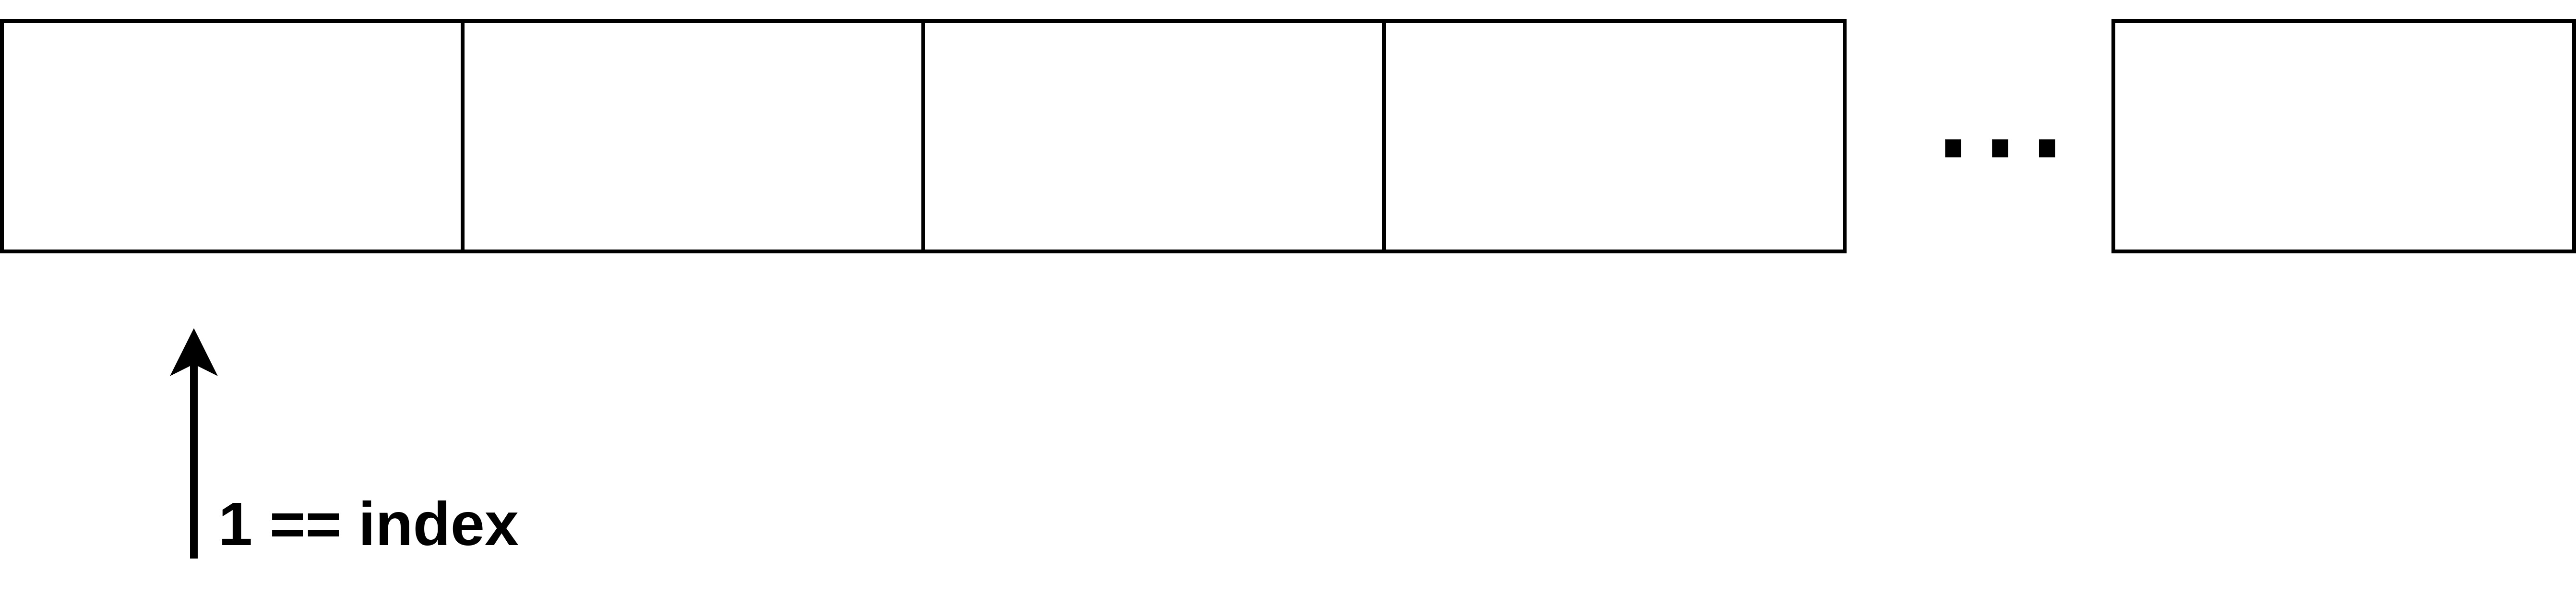
\includegraphics[scale=0.04]{messagequeue.eps}
    \caption{\label{fig:singlemq}A single message queue}
\end{figure}
    \begin{figure}[H]
    \centering
    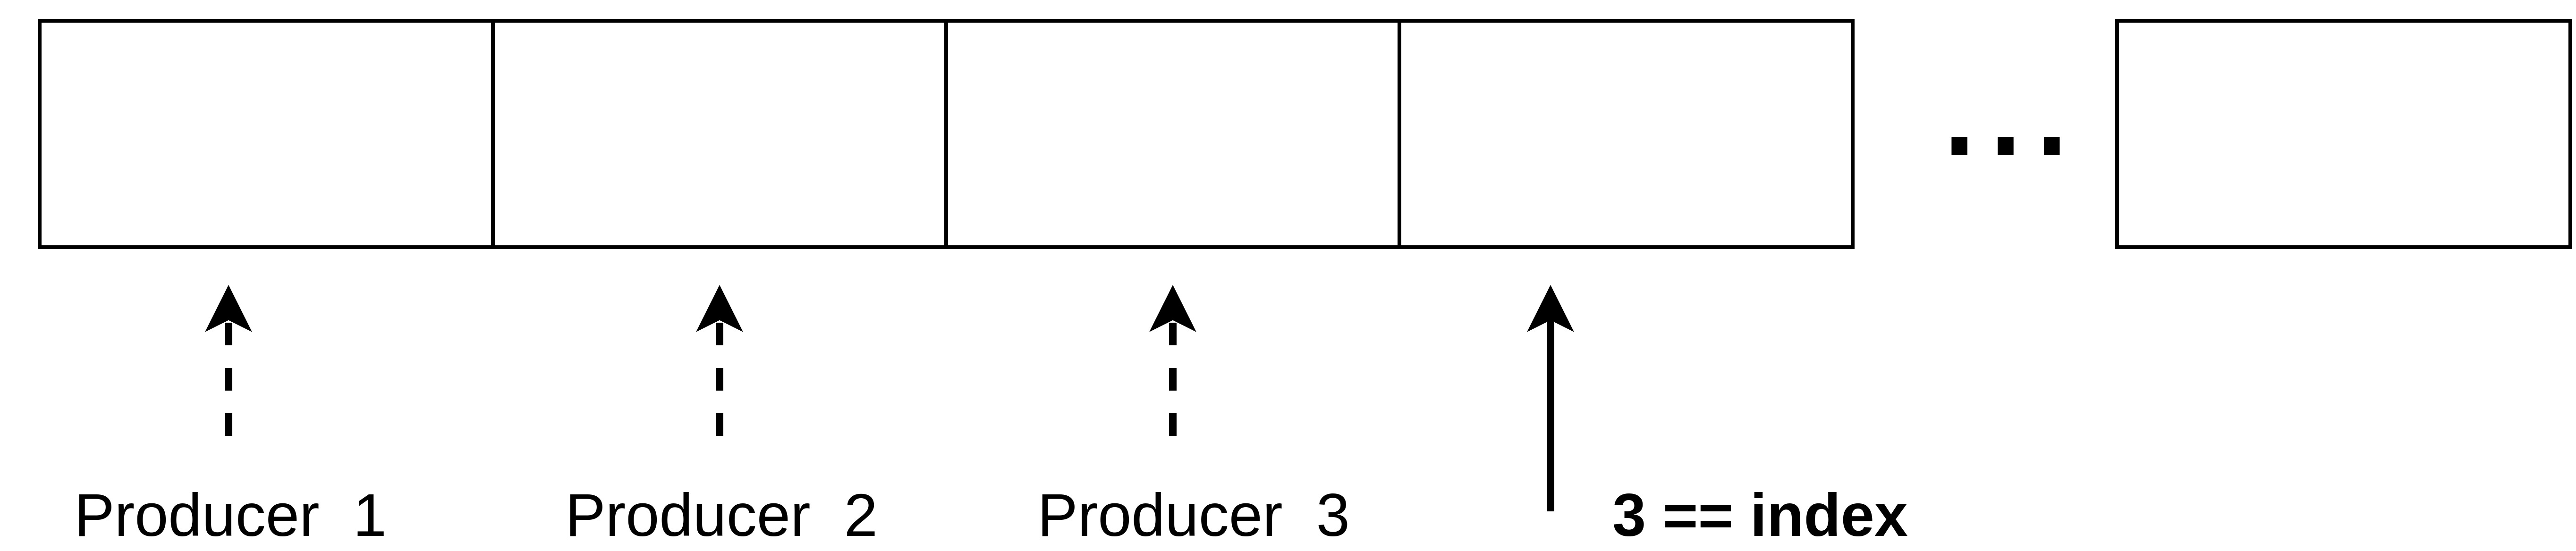
\includegraphics[scale=0.04]{afterfetchandadd.eps}
    \caption{\label{fig:afterfa}After three fetch-and-add operations}
\end{figure}
\end{subfigures}

\noindent
There are only one consumer (\textit{i.e.}, \textit{KM agent}) but many
producers (\textit{i.e.}, the hooked processes). Upon sending message,
producers will advance the \textit{index} using the fetch-and-add atomic
operation such that every producer get its own slot. This process is
illustrated in Figure~\ref{fig:afterfa}. Every producer simply take the
module of the result of the fetch-and-add operation on the size of the queue
to avoid index overflow. To collect messages from producers, the \textit{KM
agent} periodically polls all the message queues and read the slots one by
one.\\ 

\noindent
\textbf{Synchronization Between A Consumer and A Producer}. In each slot, a
flag variable is used to synchronize between a consumer and any one of the
producers. Before collecting information in any slot, the consumer will check
whether that flag is set to SLOTFULL. If so, it will go ahead reading the
slot, after which the flag is set to SLOTEMPTY. Before writing to any slot,
the producer will check whether whether that flag is set to SLOTEMPTY. If so,
it will go ahead writing information in that slot, after which the flag is
set to SLOTFULL. Because there is only one consumer, there is no need to use
any atomic operation on that flag. A ordinal read and write will suffices.
Therefore, synchronization between the consumer and producers is cheep and
fast.\\

\noindent
\textbf{Synchronization Among Producers}. Synchronization among producers is
more tricky because simply taking the modulo of the result of the
fetch-and-add operation on the size of the queue (to avoid index overflow)
will probably result in two process collict in the same slot. To avoid this,
an internal lock is setup and atomic operations are used to operation on it.
This internal lock is a 8 bit integer so operation on it should be fast. The
advantages of using this kind of home-brew lock with atomic operation is not
only its speed and simplicity, but also that it can be turned into a robust
lock so that any process which accidentally dies while holding this lock will
not prevent the corresponding slot being used by other process. To achieve
this robustness, we use fetch-and-add atomic operation for locking and take
advantage of the automatic wrap-around effect of an unsigned integer. When a
process exits without unlocking this lock, other processes which try to lock
this lock with fetch-and-add operation will eventually overflow the
underlying unsigned integer to zero, effectively unlocking it. Because we use
a single byte as the underlying lock, 255 times of fetch-and-add would
suffice. And because the message queue is long enough, the overflow will not
happen too fast. The overall algorithm for this process is shown in
Algorithm~\ref{algo:syncproducers}.

% make \Return begin on a newline
\let\oldReturn\Return
\renewcommand{\Return}{\State\oldReturn}
\begin{algorithm}
\caption{Synchronization Among Producers}\label{algo:syncproducers}
\begin{algorithmic}[1]     % 1 for line number for every 1 line
\Procedure{SyncProducer}{}
    \If {$flag = SLOTFULL$} \Return false \EndIf
    \If {$0 \ne fetch-and-add(lock)$} \Return false \EndIf
    \State copy message to slot
    \State unset flag and lock altogether
    \Return true
\EndProcedure
\end{algorithmic}
\end{algorithm}


\subsection{Forward Tracing} \label{sec:fwtracing}

Once we have data of all relevant events, we can chain up events to get a
clear picture of how those events relate to each other, and more importantly,
how a piece of data is transfered with hosts and across hosts.  This procedure
starts by the data under monitor (which we call the \textit{tracingpoint}),
and populates by a breath first search.

An example of this is given at Figure~\ref{fig:filetransfermodel}. The event
order of it is:

\begin{enumerate}
    \item Process A read file \textit{/etc/passwd} and then open a socket
        \textit{/var/sock.1} at time \textit{T1}.
    \item Process A fork a process B and write data to \textit{/var/sock.1} at
        time \textit{T2}.
    \item Process B read data from \textit{/var/sock.1} at time \textit{T3}. 
    \item Process B connect a remote host at address
        \textit{192.168.20.344:6677} at time \textit{T4}.
    \item Process C accept the connection from B at time \textit{T5}.
\end{enumerate}

where time \textit{T1-5} are in ascending order.\\

Clearly these events are suspicious and should be put under administrators'
attention.

To perform forward tracing, it is required that file \textit{/etc/passwd} is
%TODO How should we call that "monitor list"?
added to the monitor list at the very beginning. If it is added, then process
A's read operation will be intercepted and its subsequent operations of
opening a socket, forking a subprocess and writing data to that socket will
all be under interception. Because the socket \textit{/var/sock.1} was opened
by process A, which is under interception, the path \textit{/var/sock.1} will
be added to the monitor list automatically by our interception code, such that
process B's read operation on it will be intercepted. The connect and accept
operations are monitored all the time so we can chain together process B and
process C's events. % TODO this is where the probability model comes in

As described in the example above, once a read or write to a file in the
monitor list is intercepted, we can start from that \textit{tracingpoint} and
perform a breath first search in our database to get a clear picture of how a
piece of data is manipulated and transfered. Moreover, with a proper login
control system, we can have information of which user starts which process at
which time, and therefore can which users are involved in this series of
events.

\subsection{DSO Runtime Injection} \label{sec:dso}

Since the whole system works by libc interception, processes which are already
running at the time of deployment will not be affected. To address this we can
either reboot the machines or inject a library (in ELF format) into the memory
space of the running process and change relevant function pointers to have
them point to the corresponding pointers in the injected library. Since
rebooting machines is not a universal solution and can do harm to many
time-sensitive services, we develop the DSO runtie injection technique.
Besides, being able to dynamically inject a dynamic shared object at runtime
allows the system adminstrators to \textit{partially} deploy the system. For
example, some adminstrators might not want to intercept a long-running
\textit{logind} process. With the DSO runtime injection technique, they are
free to do so.

The technique of DSO runtime injection consists of 1) injecting the shared
object into the memory of a running process and 2) change relevant function
pointers (in libc) to point to that in the injected object. Injecting the
shared object can be done by using the \textit{ptrace(2)} system
call~\cite{ptrace:2017}, as in most debuggers. Changinng function pointers can
be done by analysing the current process's ELF structure, finding the correct
pointers and changing them. The procedure of doing this is straightforward,
but it is not easy to doing it in a safe way that does not crash a running
program, especially when the program is compiled as PIE with
RELRO~\cite{something}. Also, we have to guarantee that all our operations are
safe multithread-safe and async-signal-safe such that the behavior of a
running process will not be affected.

TODO more detail here.

\subsection{Optimization} \label{sec:optm}

Describe the optimization techniques we use.

\section{Experiments and Evaluation}

1. the data output (how things are traced)

2. the performance (overhead)

\section{Future work}

\section{Acknowledgments}

A polite author always includes acknowledgments.  Thank everyone,
especially those who funded the work. 

\section{Availability}

It's great when this section says that MyWonderfulApp is free software, 
available via anonymous FTP from

\begin{center}
{\tt ftp.site.dom/pub/myname/Wonderful}\\
\end{center}

Also, it's even greater when you can write that information is also 
available on the Wonderful homepage at 

\begin{center}
{\tt http://www.site.dom/\~{}myname/SWIG}
\end{center}

Now we get serious and fill in those references.  Remember you will
have to run latex twice on the document in order to resolve those
cite tags you met earlier.  This is where they get resolved.
We've preserved some real ones in addition to the template-speak.
After the bibliography you are DONE.

{\footnotesize \bibliographystyle{acm}
\bibliography{km.bib}}

\end{document}
